% A rotation (generated by figs_c2ch03.py).
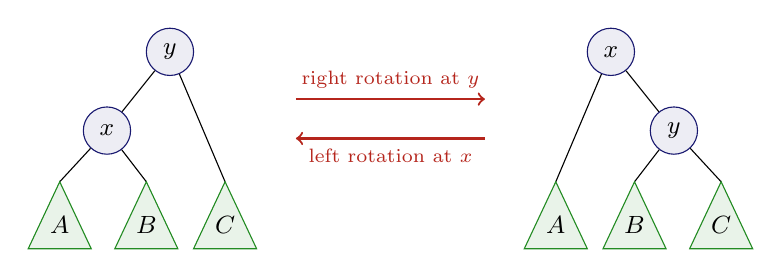
\begin{tikzpicture}[x=1cm,y=1cm,every node/.style={font=\small}]
\tikzset{nd/.style={circle,draw=MidnightBlue,fill=MidnightBlue!8,inner sep=1.5pt,minimum size=0.6cm}}
\node[nd] (y1) at (1.6,0) {$y$};
\node[nd] (x1) at (0.8,-1.0) {$x$};
\draw (y1) -- (x1);
\draw (y1) -- (2.3,-1.65);
\draw (x1) -- (0.2,-1.65);
\draw (x1) -- (1.3,-1.65);
\draw[ForestGreen,fill=ForestGreen!10] (0.20,-1.65) -- (-0.20,-2.50) -- (0.60,-2.50) -- cycle;
\node at (0.20,-2.20) {$A$};
\draw[ForestGreen,fill=ForestGreen!10] (1.30,-1.65) -- (0.90,-2.50) -- (1.70,-2.50) -- cycle;
\node at (1.30,-2.20) {$B$};
\draw[ForestGreen,fill=ForestGreen!10] (2.30,-1.65) -- (1.90,-2.50) -- (2.70,-2.50) -- cycle;
\node at (2.30,-2.20) {$C$};
\draw[->,thick,BrickRed] (3.2,-0.6) -- node[above,font=\scriptsize] {right rotation at $y$} (5.6,-0.6);
\draw[<-,thick,BrickRed] (3.2,-1.1) -- node[below,font=\scriptsize] {left rotation at $x$} (5.6,-1.1);
\node[nd] (x2) at (7.2,0) {$x$};
\node[nd] (y2) at (8.0,-1.0) {$y$};
\draw (x2) -- (y2);
\draw (x2) -- (6.5,-1.65);
\draw (y2) -- (7.5,-1.65);
\draw (y2) -- (8.6,-1.65);
\draw[ForestGreen,fill=ForestGreen!10] (6.50,-1.65) -- (6.10,-2.50) -- (6.90,-2.50) -- cycle;
\node at (6.50,-2.20) {$A$};
\draw[ForestGreen,fill=ForestGreen!10] (7.50,-1.65) -- (7.10,-2.50) -- (7.90,-2.50) -- cycle;
\node at (7.50,-2.20) {$B$};
\draw[ForestGreen,fill=ForestGreen!10] (8.60,-1.65) -- (8.20,-2.50) -- (9.00,-2.50) -- cycle;
\node at (8.60,-2.20) {$C$};
\end{tikzpicture}
